% Copyright 2004 by Till Tantau <tantau@users.sourceforge.net>.
%

% In principle, this file can be redistributed and/or modified under
% the terms of the GNU Public License, version 2.
%
% However, this file is supposed to be a template to be modified
% for your own needs. For this reason, if you use this file as a
% template and not specifically distribute it as part of a another
% package/program, I grant the extra permission to freely copy and
% modify this file as you see fit and even to delete this copyright
% notice. 

\documentclass{beamer}

\usepackage{enumitem}
%encoding for portuguese
%--------------------------------------
\usepackage[utf8]{inputenc}
\usepackage[T1]{fontenc}
\usepackage[brazil]{babel}
%--------------------------------------

% para incluir imagens
\usepackage{graphicx}
\graphicspath{{images/}}
%%%%%%%%%%%%%%%%%%%%%

%
% There are many different themes available for Beamer. A comprehensive
% list with examples is given here:
% http://deic.uab.es/~iblanes/beamer_gallery/index_by_theme.html
% You can uncomment the themes below if you would like to use a different
% one:
%\usetheme{AnnArbor}
%\usetheme{Antibes}
%\usetheme{Bergen}
%\usetheme{Berkeley}
%\usetheme{Berlin}
%\usetheme{Boadilla}
%\usetheme{boxes}
%\usetheme{CambridgeUS}
%\usetheme{Copenhagen}
%\usetheme{Darmstadt}
%\usetheme{default}
%\usetheme{Frankfurt}
%\usetheme{Goettingen}
%\usetheme{Hannover}
%\usetheme{Ilmenau}
%\usetheme{JuanLesPins}
%\usetheme{Luebeck}
%\usetheme{Madrid}
%\usetheme{Malmoe}
%\usetheme{Marburg}
%\usetheme{Montpellier}
%\usetheme{PaloAlto}
%\usetheme{Pittsburgh}
%\usetheme{Rochester}
%\usetheme{Singapore}
%\usetheme{Szeged}
%\usetheme{Warsaw}

\title{Entendimento dos Dados}

\date{\today}

% apenas inserido no pdf - opcional
%\subject{{por_titulo}}

% Delete this, if you do not want the table of contents to pop up at
% the beginning of each section:
%\AtBeginSection[]
%{
%  \begin{frame}<beamer>{Conteúdo}
%    \tableofcontents[currentsection, currentsubsection, subsectionstyle=show/show/hide]
%  \end{frame}
%}

% for the number of the page appear
\setbeamerfont{page number in head/foot}{size=\large}
\setbeamertemplate{footline}[frame number]

% get started
\begin{document}

\begin{frame}
  \titlepage
\end{frame}

% introductory text 
% imputação
% limpeza dos dados
% histograma dos valores
% matriz de correlação

\section{Preparação dos Dados}
\begin{frame}{Seleção dos Dados}
\begin{itemize}[itemsep=3ex]
    \item Utilização dos dados de 2000 até 2009 como treino e de 2010 até 2015 para
        testes. 
    \item Atributos que serão levados em consideração foram explicados na fase de
        entendimento dos dados: sexo, idade, UF, cotista, tipo da escola,
        curso, forma de ingresso, IRA.
\end{itemize}
\end{frame}

\begin{frame}{Construção dos Atributos Derivados}
\begin{itemize}[itemsep=3ex]
    \item Atributos derivados que serão construídos já foram definidos na fase
        anterior.
    \item A seguir, histograma mostrando a distribuição de tais atributos
\end{itemize}
\end{frame}

\begin{frame}{Histograma da Distribuição dos Atributos Derivados - Coeficiente de
    Melhora Acadêmica}
\begin{itemize}[itemsep=3ex]
        \item O coeficiente de melhora acadêmica é definido como sendo a razão entre
            as notas do semestre anterior e as notas do semestre anterior ao
            anterior.
        \item Por histograma aqui
\end{itemize}
\end{frame}

\begin{frame}{Histograma - Taxa de Aprovação (antigo)}
    \begin{figure}[!ht]
    \centering
    \includegraphics[width = 8cm]{pass_rate_old.png}
    \end{figure}
\end{frame}

\begin{frame}{Histograma - Taxa de Reprovação (antigo)}
    \begin{figure}[!ht]
    \centering
    \includegraphics[width = 8cm]{fail_rate_old.png}
    \end{figure}
\end{frame}

\begin{frame}{Histograma - Taxa de Reprovação}
    \begin{figure}[!ht]
    \centering
    \includegraphics[width = 8cm]{fail_rate.png}
    \end{figure}
\end{frame}

\begin{frame}{Histograma - Taxa de Trancamentos (antigo)}
    \begin{figure}[!ht]
    \centering
    \includegraphics[width = 8cm]{drop_rate_old.png}
    \end{figure}
\end{frame}

\begin{frame}{Histograma - Razão entre disciplinas cursadas por semestre e
    disciplinas do curso}
\begin{itemize}[itemsep=3ex]
        \item <Por histograma aqui>
\end{itemize}
\end{frame}

\begin{frame}{Histograma - Razão entre aprovações em disciplinas obrigatórias cursadas 
        por semestre e disciplinas do curso}
\begin{itemize}[itemsep=3ex]
        \item <Por histograma aqui>
\end{itemize}
\end{frame}

\begin{frame}{Taxa de Aprovação nas Disciplinas mais difíceis do Semestre}
\begin{itemize}[itemsep=3ex]
        \item <Por histograma aqui>
\end{itemize}
\end{frame}

\begin{frame}{Demais Atributos Derivados}
\begin{itemize}[itemsep=3ex]
        \item Demais atributos derivados incluem: booleano que indica se um aluno
            está ou não em condição e 
            a posição em relação ao semestre (0 caso seja o pior aluno, 1 caso seja o
            melhor).
\end{itemize}
\end{frame}

\begin{frame}{PCA}
\begin{itemize}[itemsep=3ex]
    \item Utilização da técnica PCA (Principal Component Analysis) para verificar se
        features estão demasiadamente relacionados. 
\end{itemize}
\end{frame}

\begin{frame}{Limpeza dos Dados}
\begin{itemize}[itemsep=3ex]
    \item Optou-se por não considerar features nos quais mais de 60\% das entradas
        fossem missing values.
    \item Descartou-se assim o feature raça.
\end{itemize}
\end{frame}

\begin{frame}{Limpeza dos Dados}
\begin{itemize}[itemsep=3ex]
    \item Para o caso de atributos que podem apresentar missing values, foi feita
        imputação (exemplo: coeficiente de melhora acadêmica).
    \item Assim, caso haja missing value coloca-se a média do feature. 
\end{itemize}
\end{frame}

\begin{frame}{Integração dos Dados}
\begin{itemize}[itemsep=3ex]
    \item Dados originais da SIGRA foram integrados com a informação dos currículos
        antigos e novos dos cursos, de modo a saber quais matérias são obrigatórias. 
\end{itemize}
\end{frame}

\begin{frame}{Transformação dos dados}
\begin{itemize}[itemsep=3ex]
    \item Utilização de dummy variables para representar dados categóricos.  
\end{itemize}
\end{frame}



% raw data
\begin{frame}{Propriedades Gerais dos Dados - Sexo}
    \begin{figure}[!ht]
        \centering
        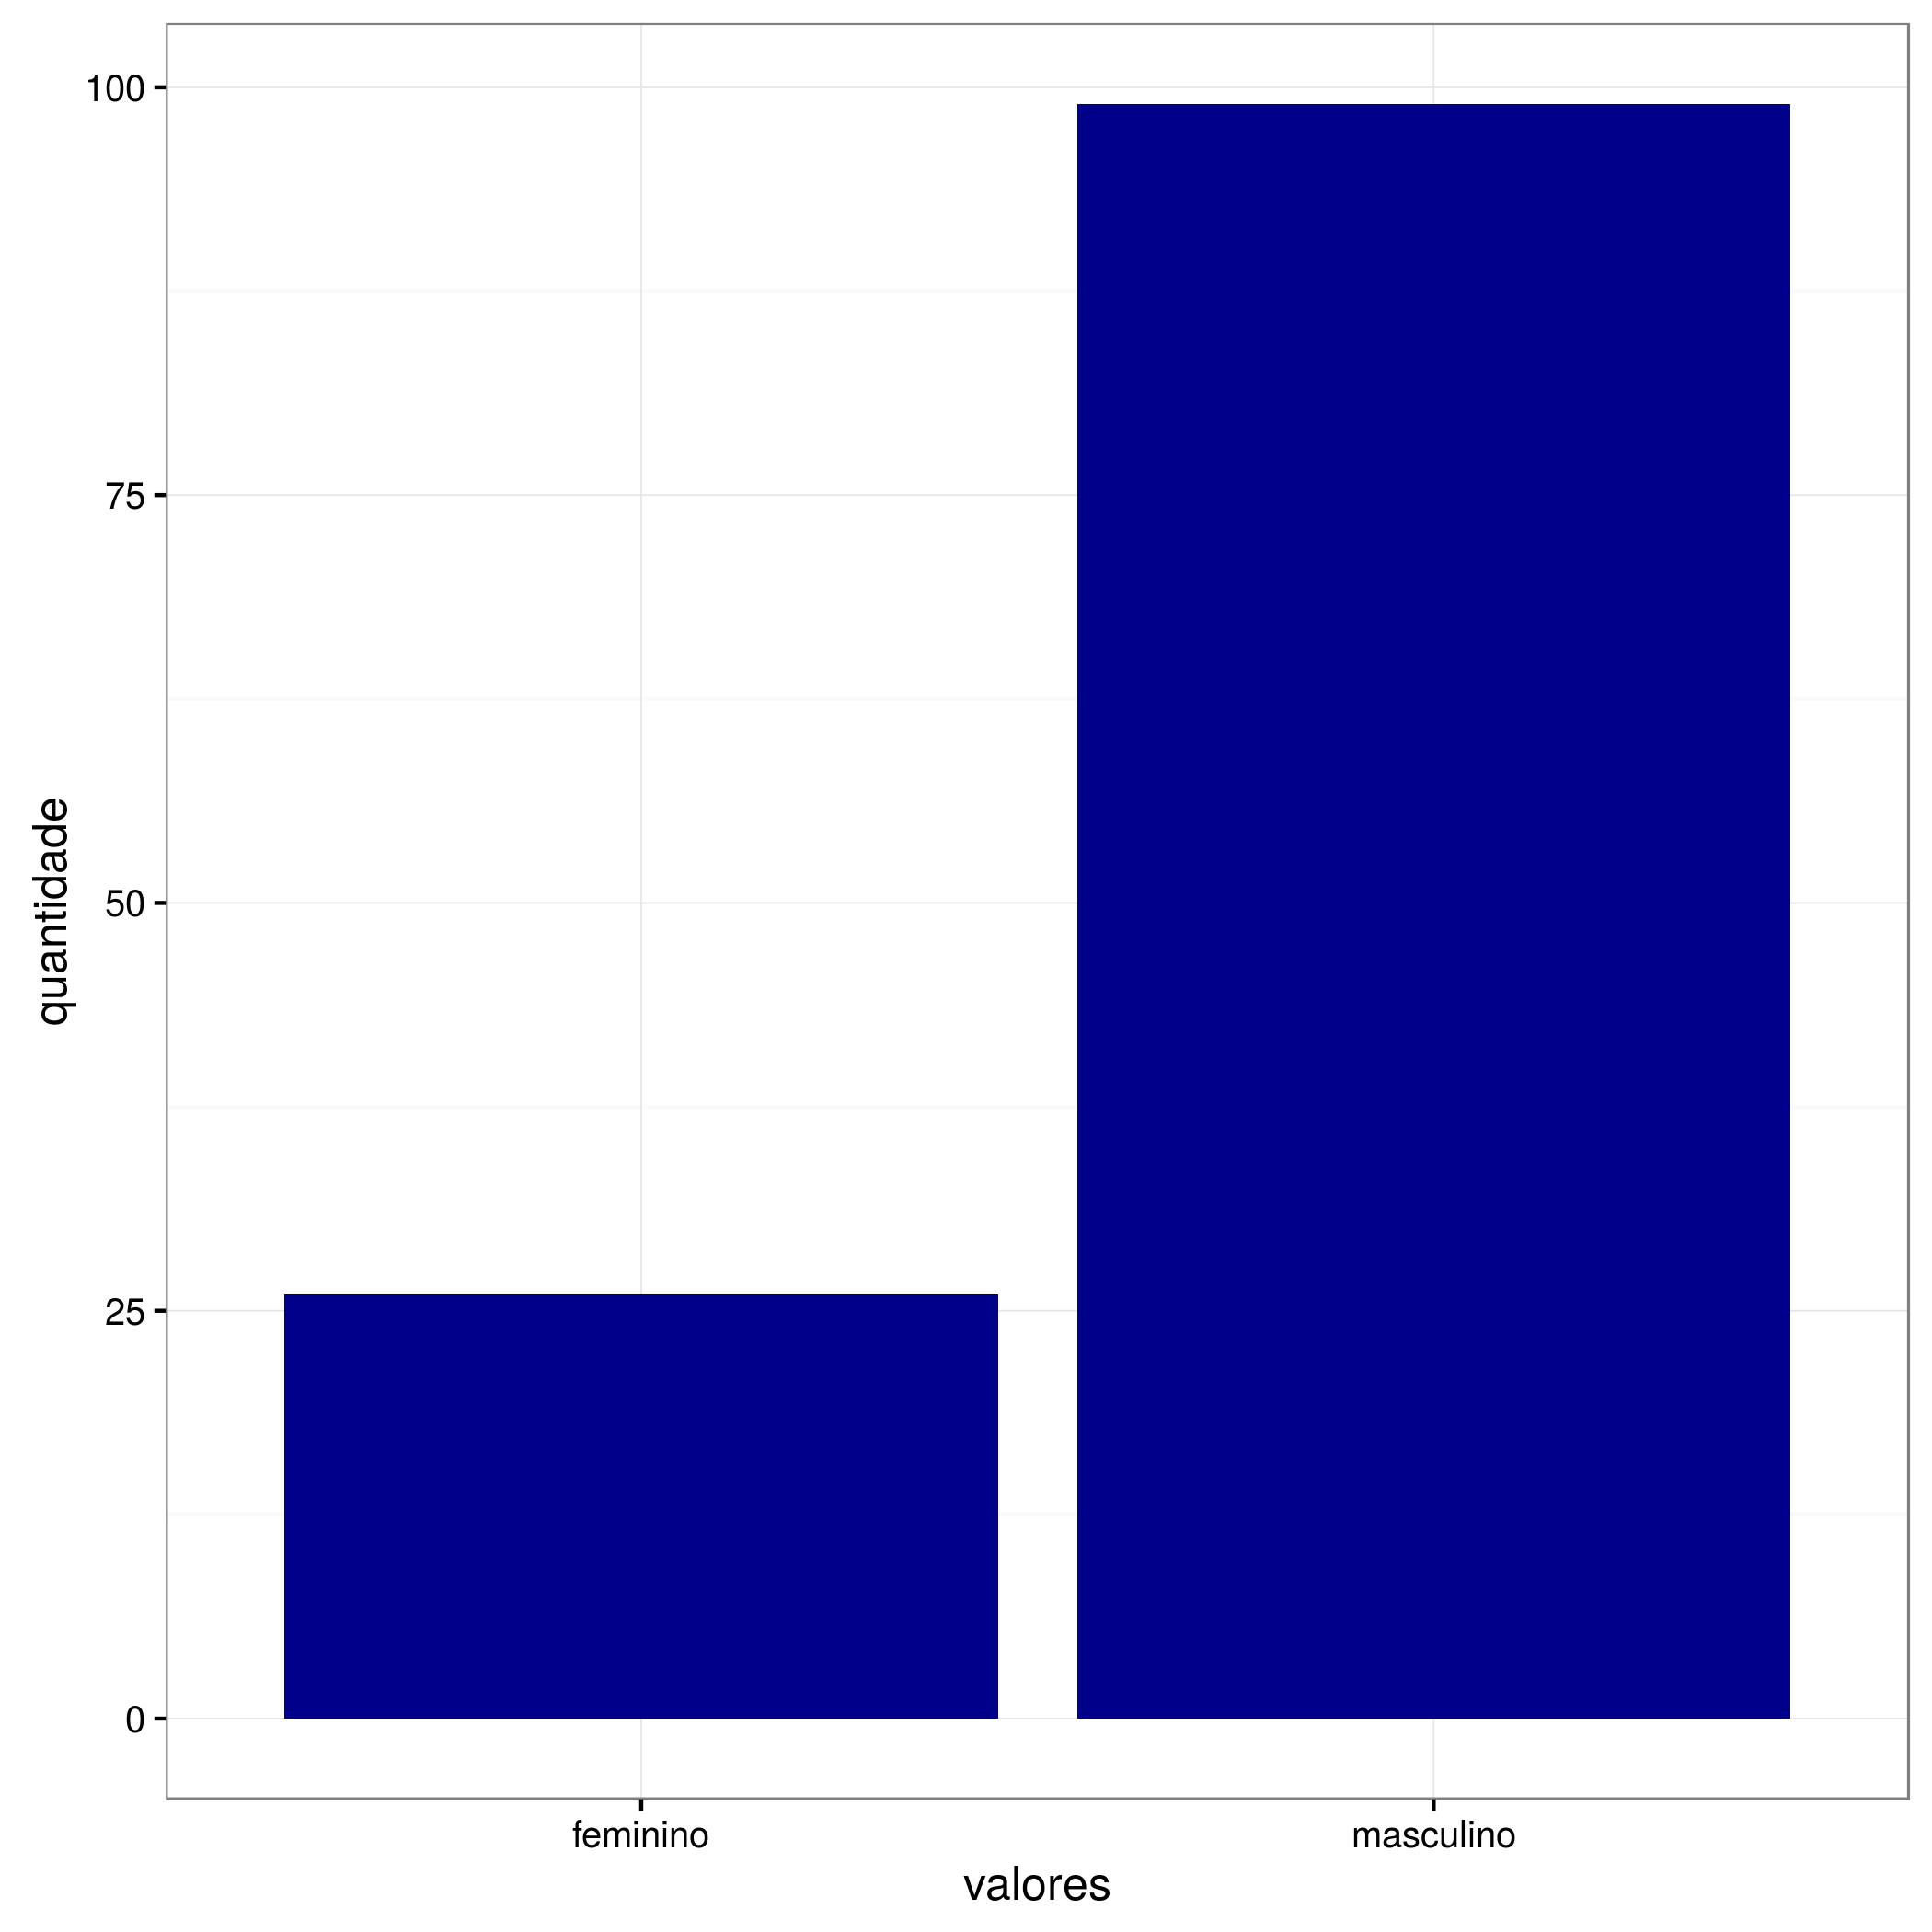
\includegraphics[width = 8cm]{sex.png}
    \end{figure}
\end{frame}

\begin{frame}{Propriedades Gerais dos Dados - Idade ao entrar}
    \begin{figure}[!ht]
        \centering
        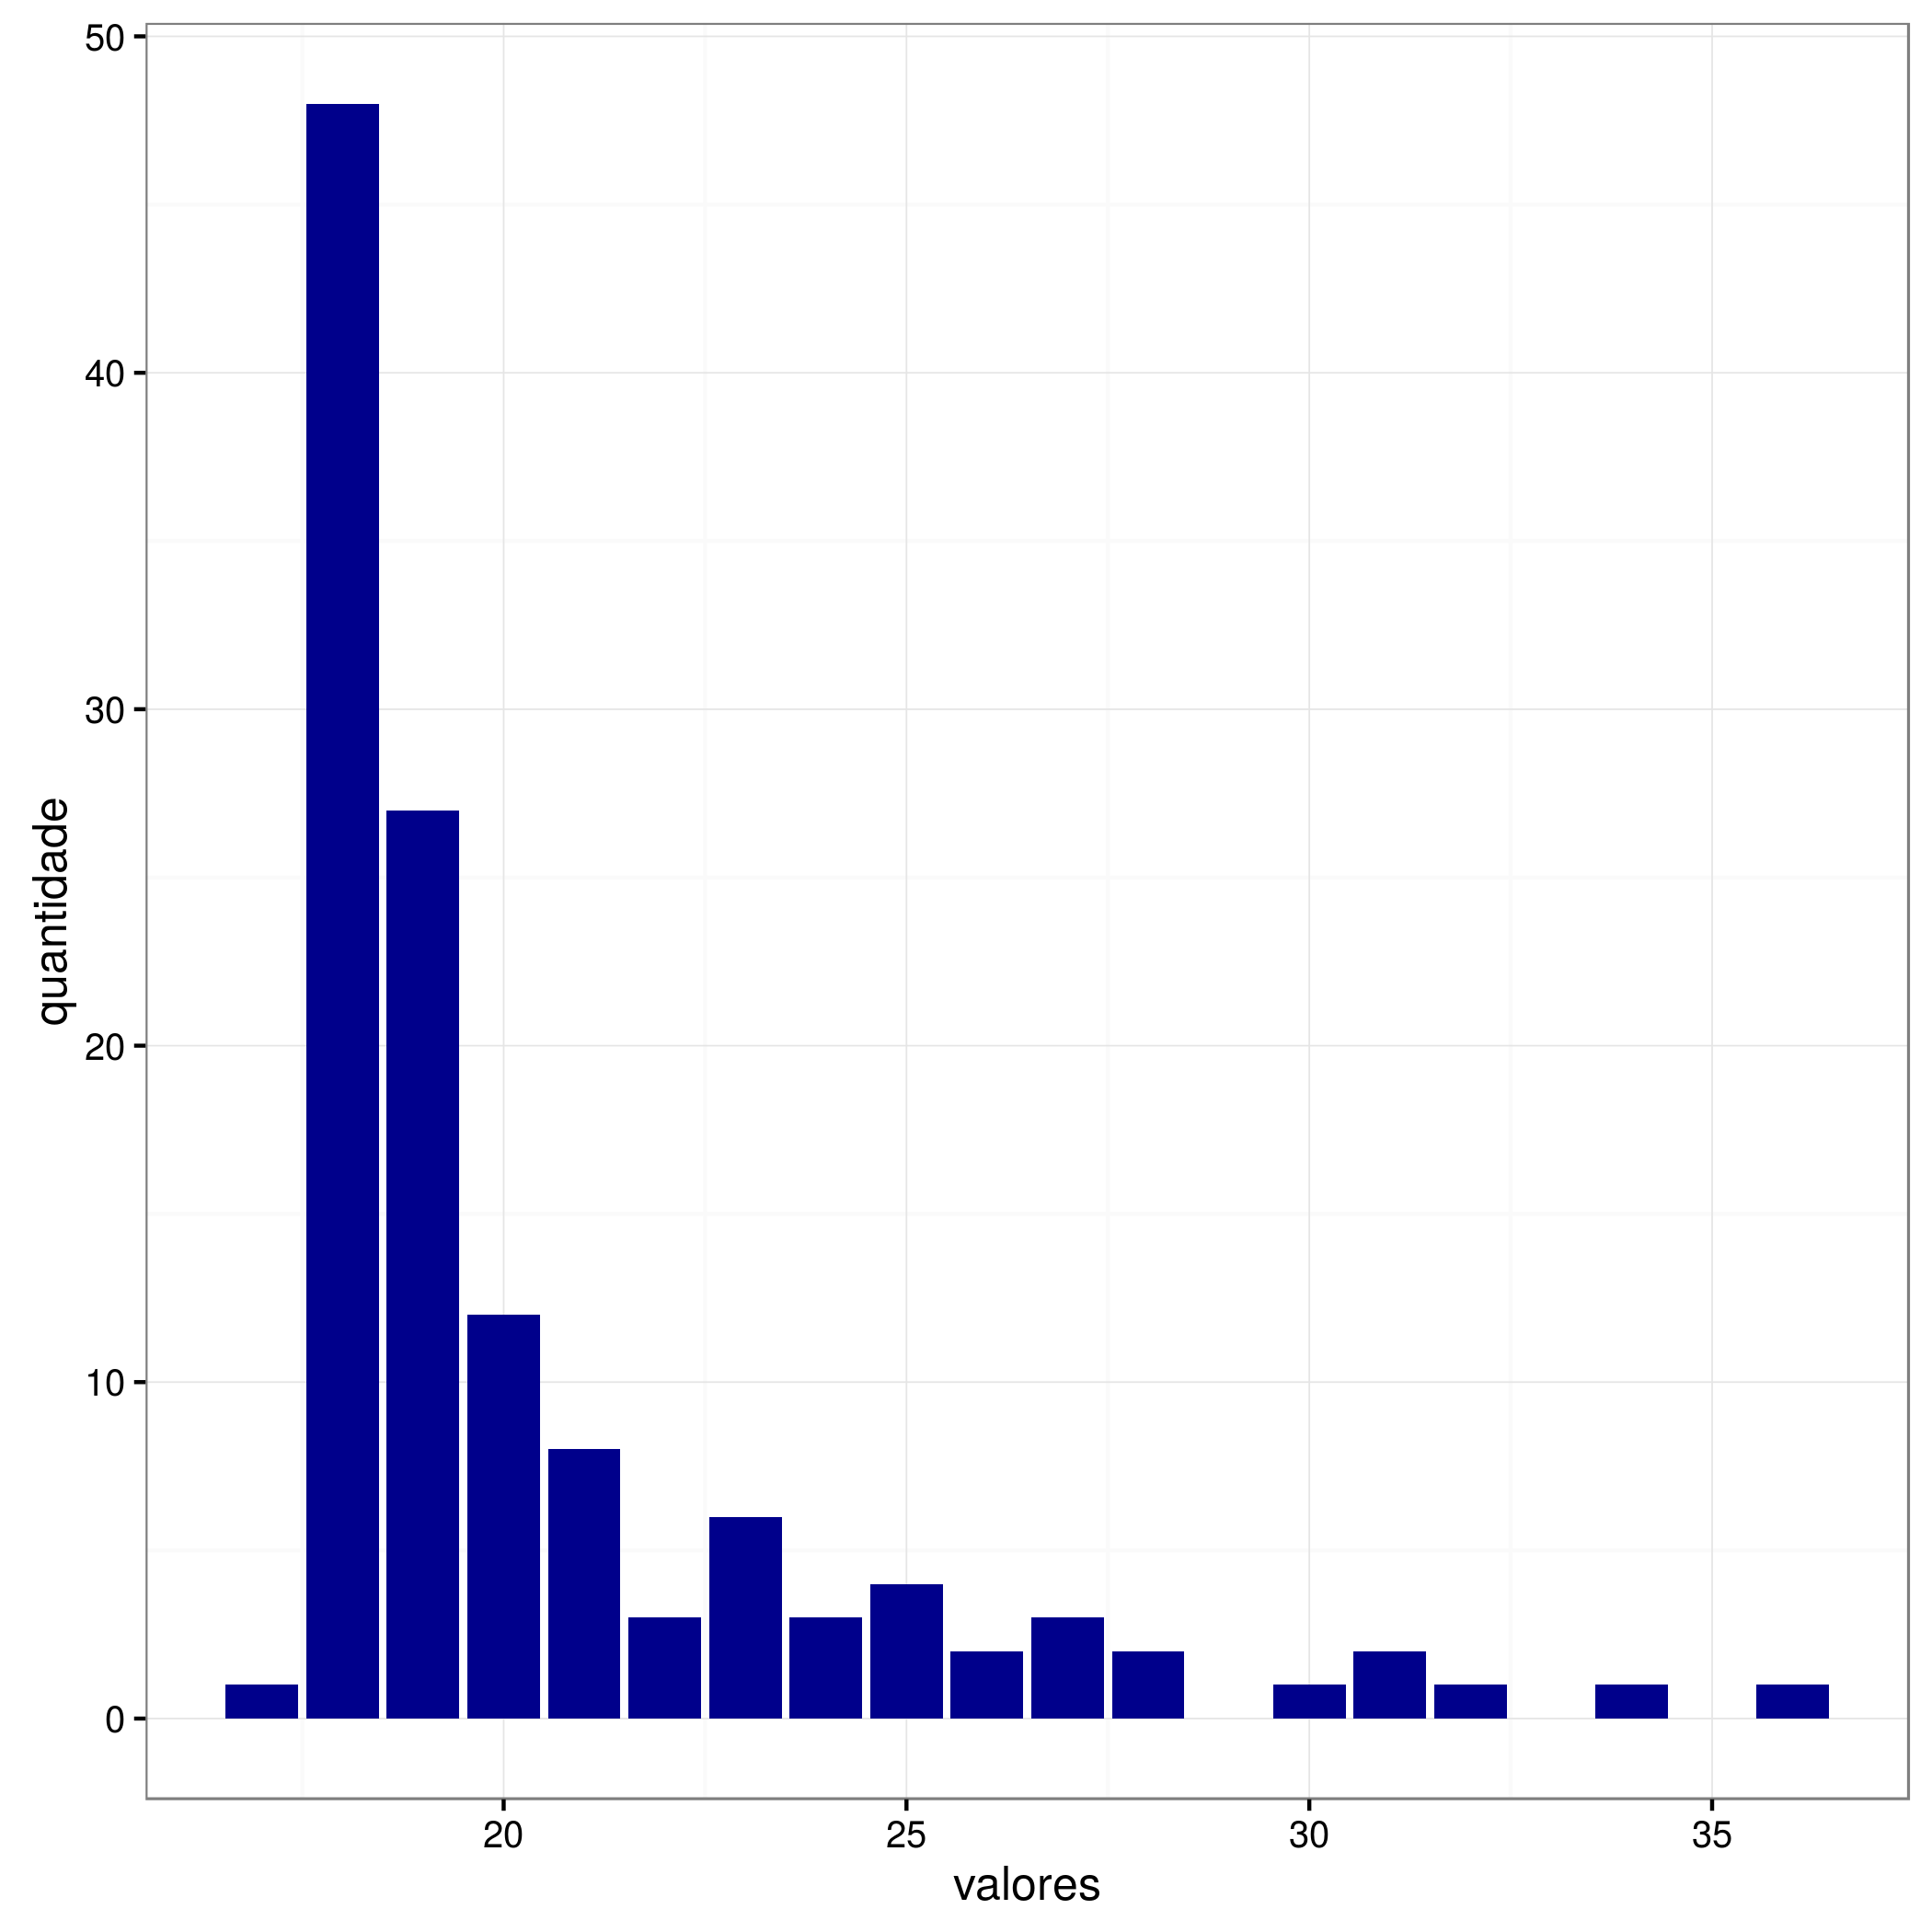
\includegraphics[width = 8cm]{age.png}
    \end{figure}
\end{frame}

\begin{frame}{Propriedades Gerais dos Dados - Residente do Local}
    \begin{figure}[!ht]
        \centering
        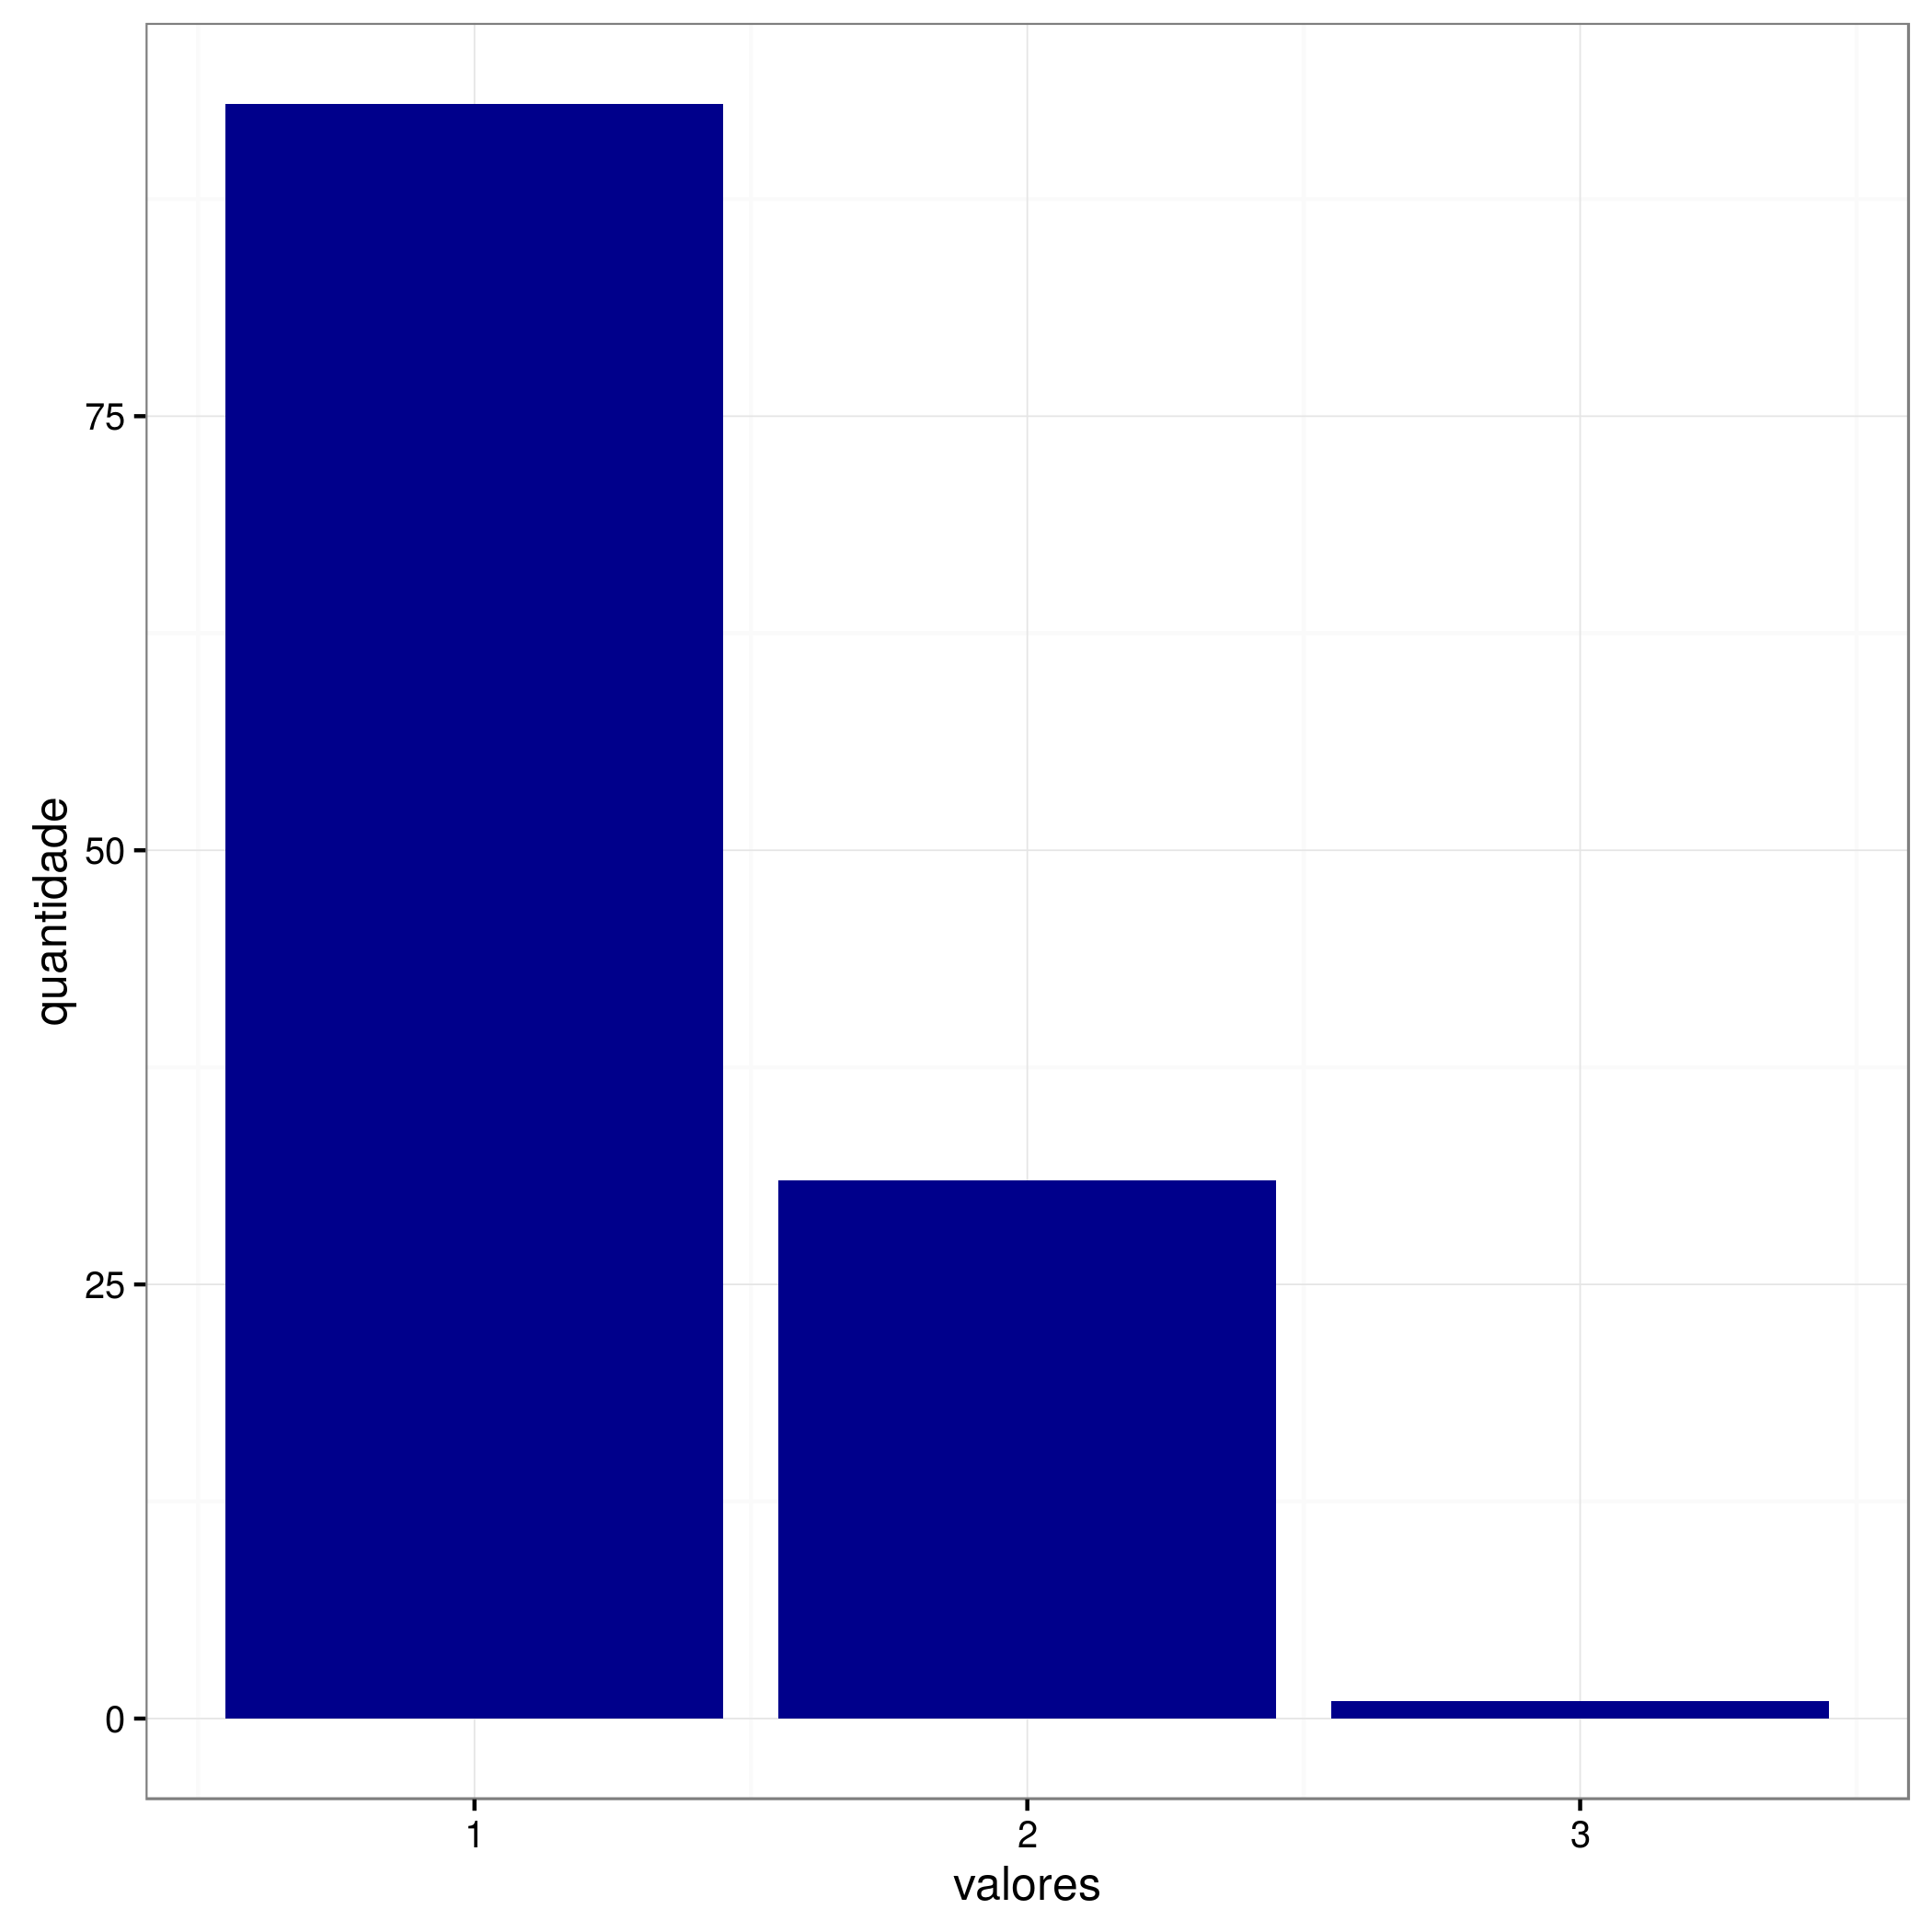
\includegraphics[width = 8cm]{local.png}
    \end{figure}
\end{frame}

\begin{frame}{Propriedades Gerais dos Dados - Cotista}
    \begin{figure}[!ht]
        \centering
        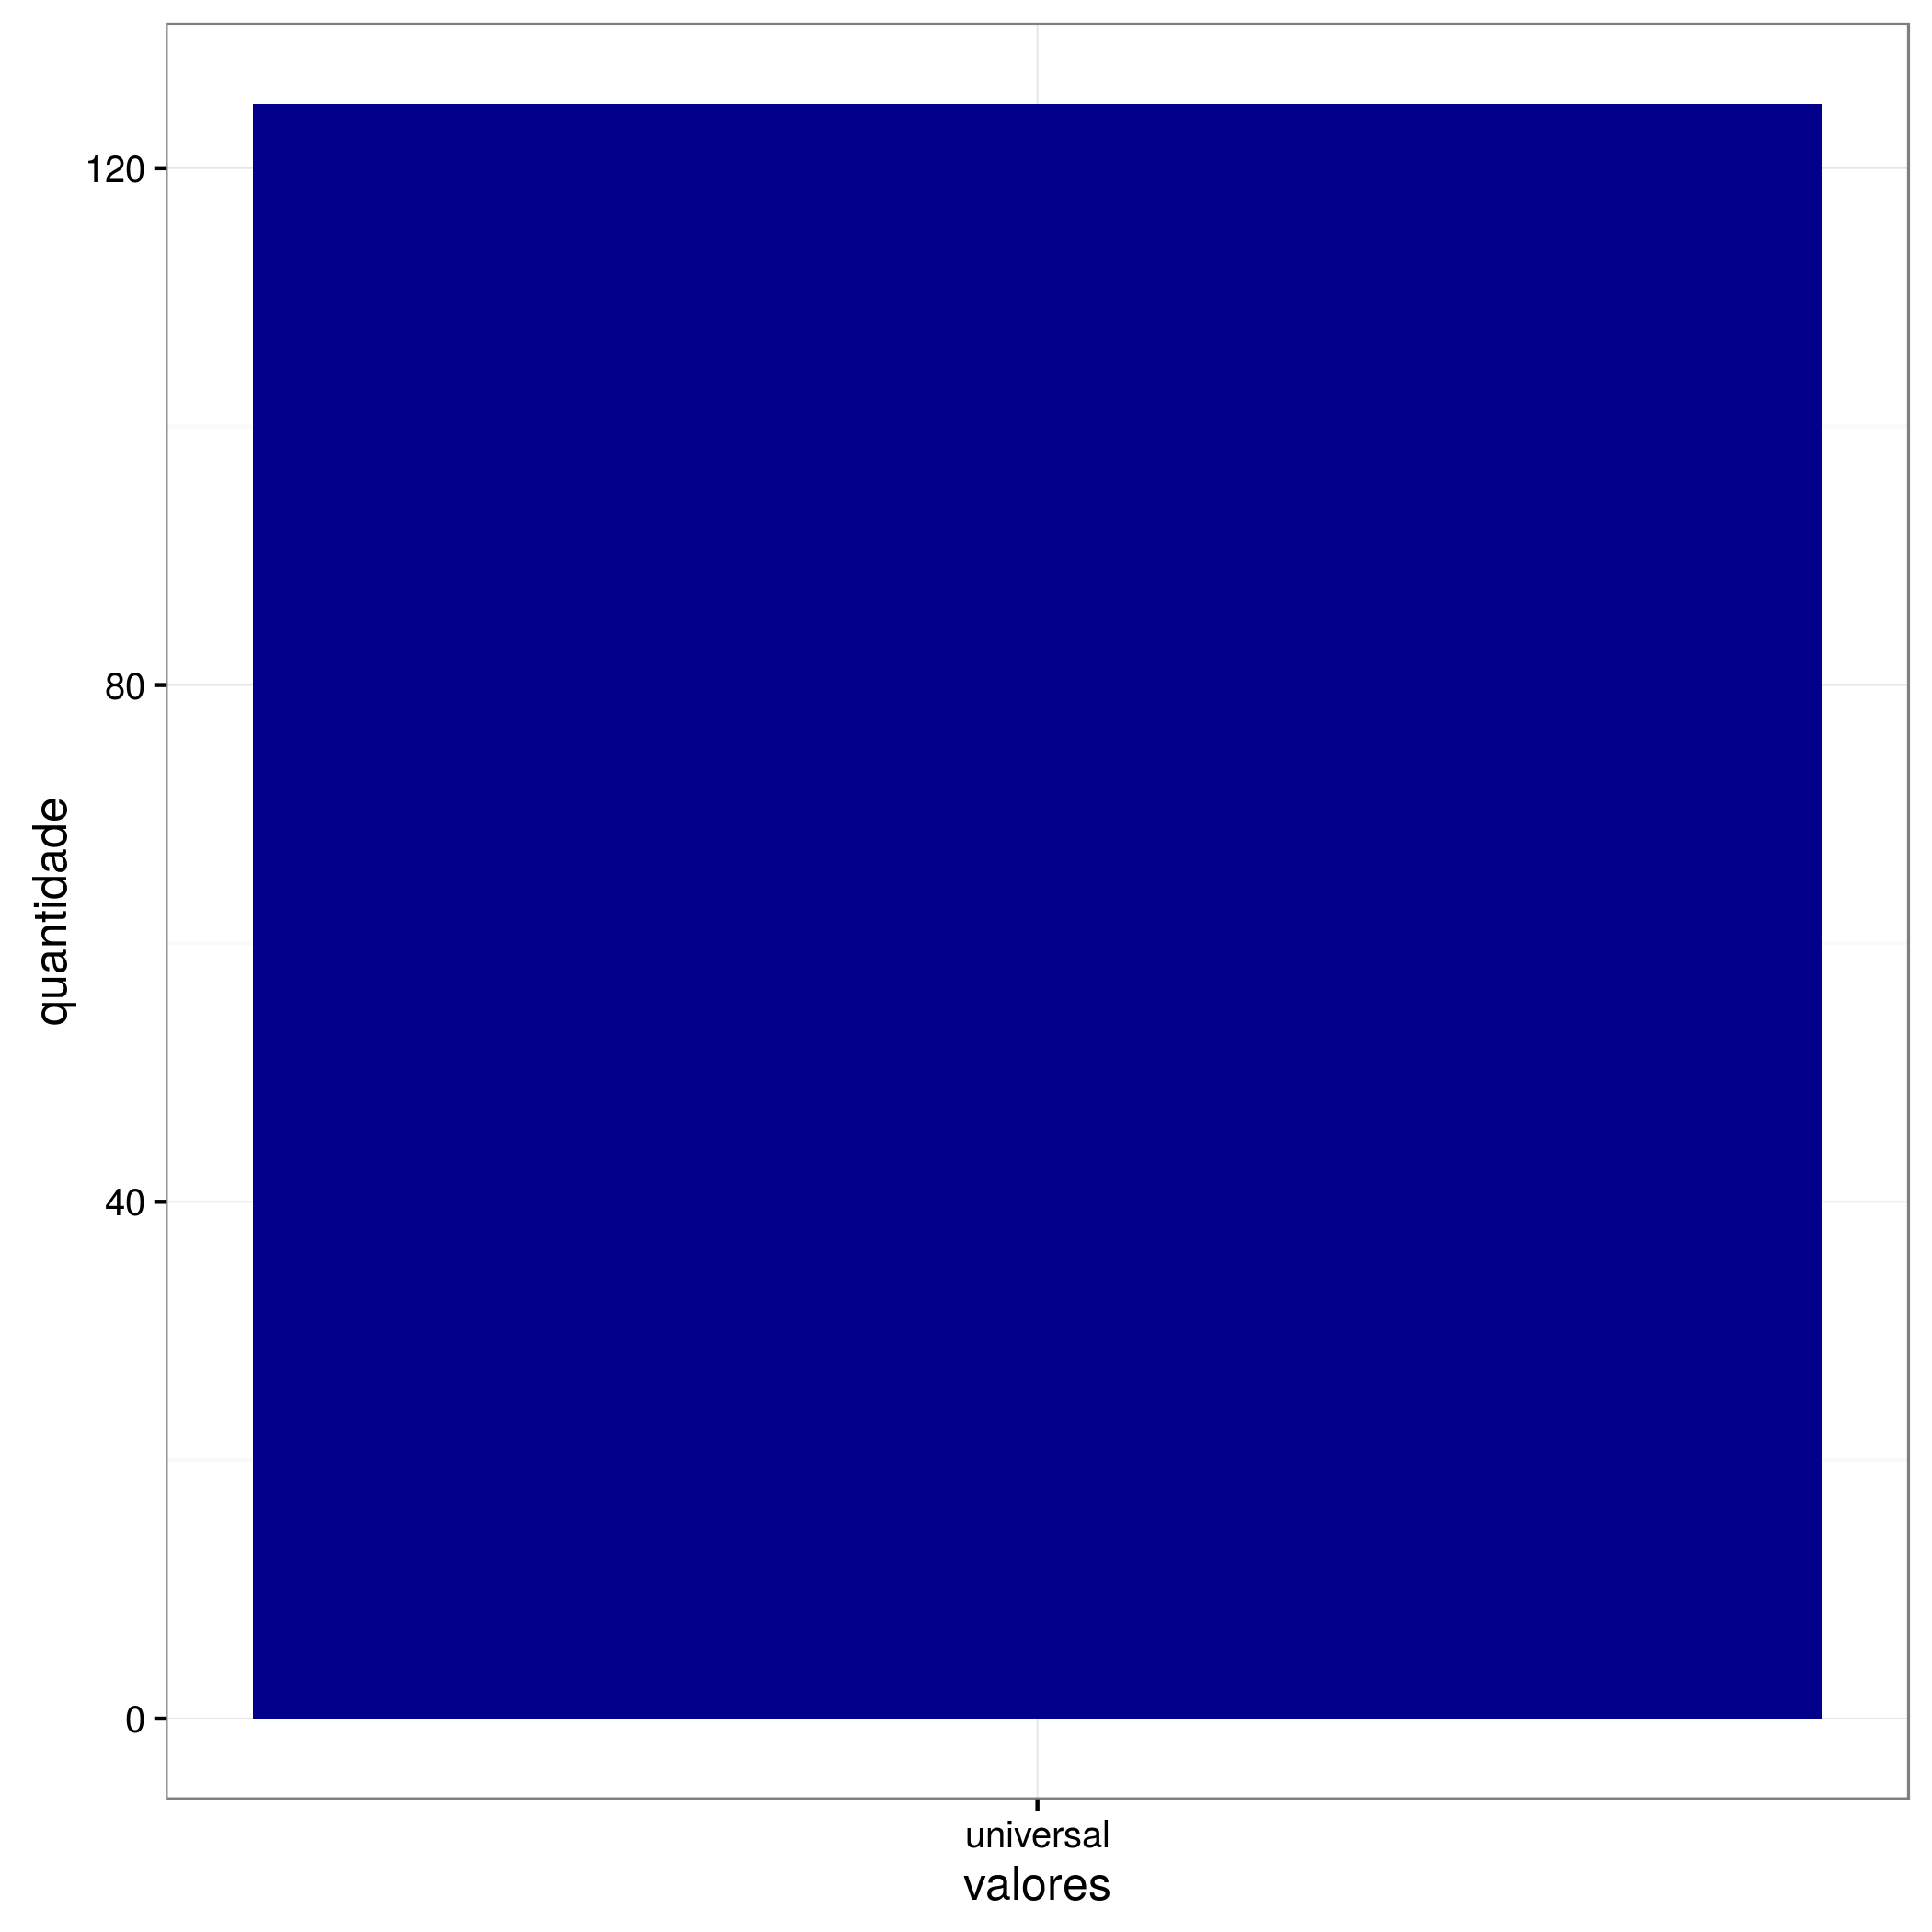
\includegraphics[width = 8cm]{quota.png}
    \end{figure}
\end{frame}

\begin{frame}{Propriedades Gerais dos Dados - Tipo da Escola}
    \begin{figure}[!ht]
        \centering
        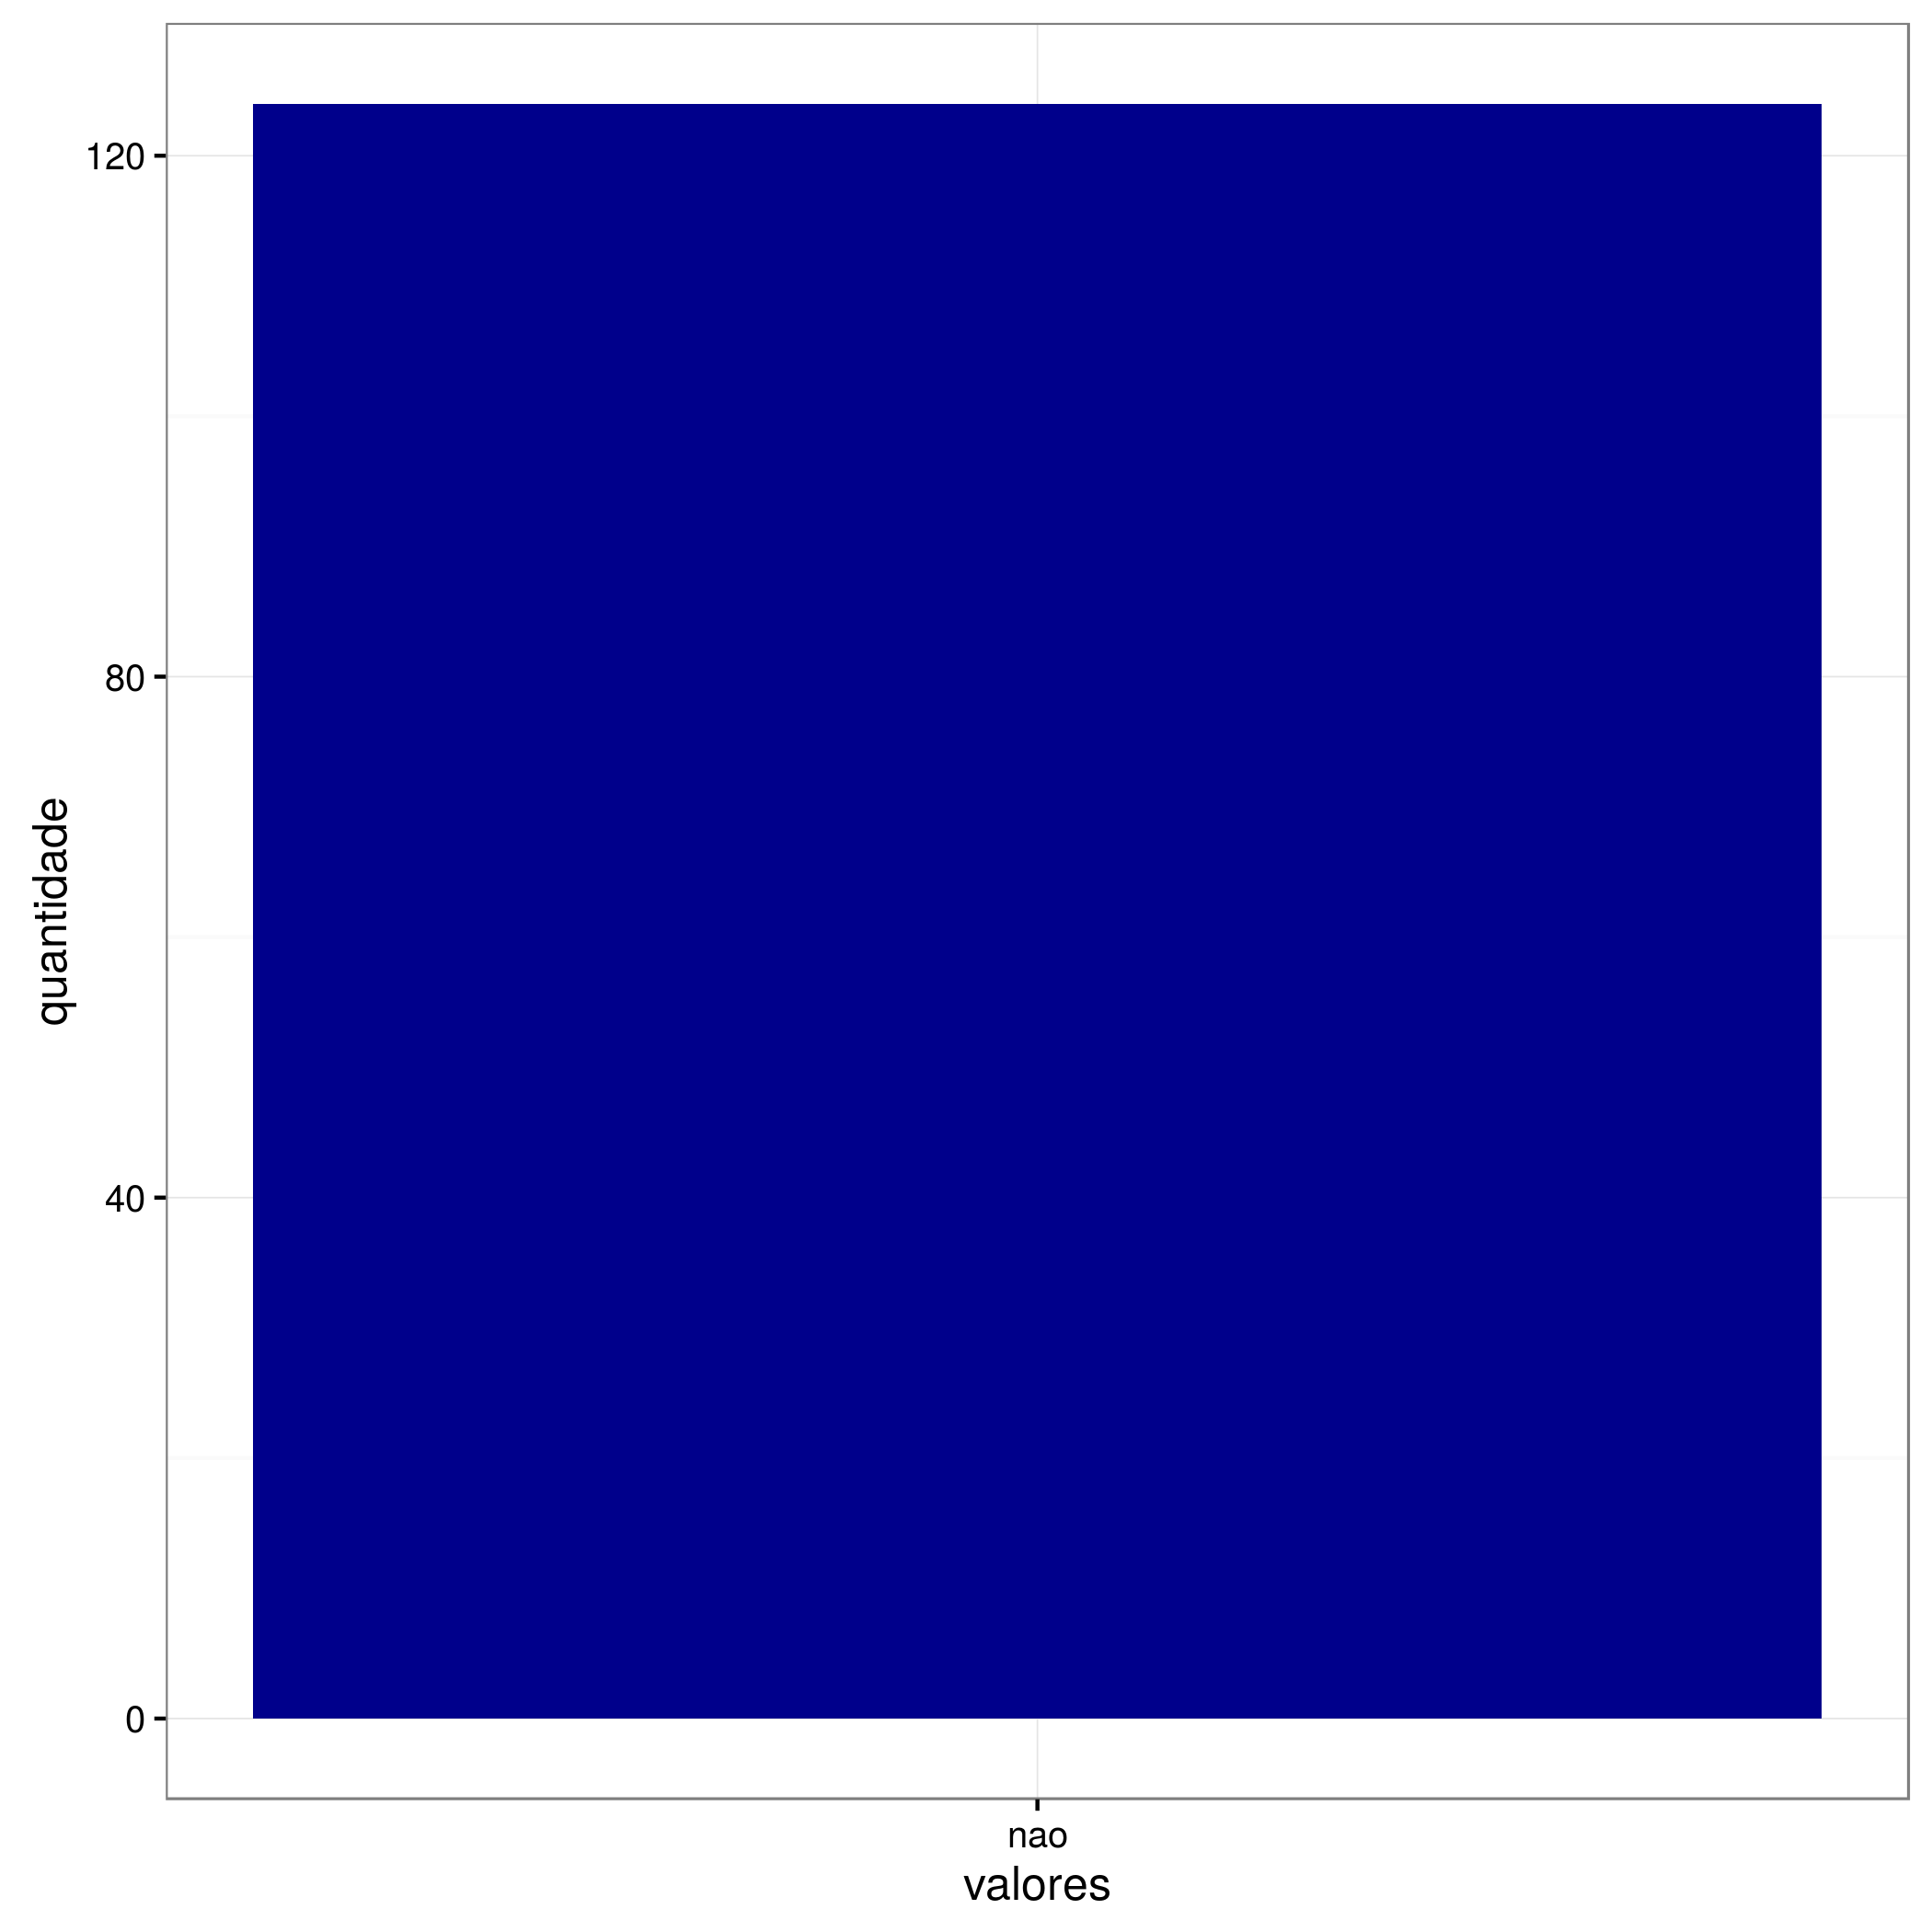
\includegraphics[width = 8cm]{school_type.png}
    \end{figure}
\end{frame}

\begin{frame}{Propriedades Gerais dos Dados - Raça}
    \begin{figure}[!ht]
        \centering
        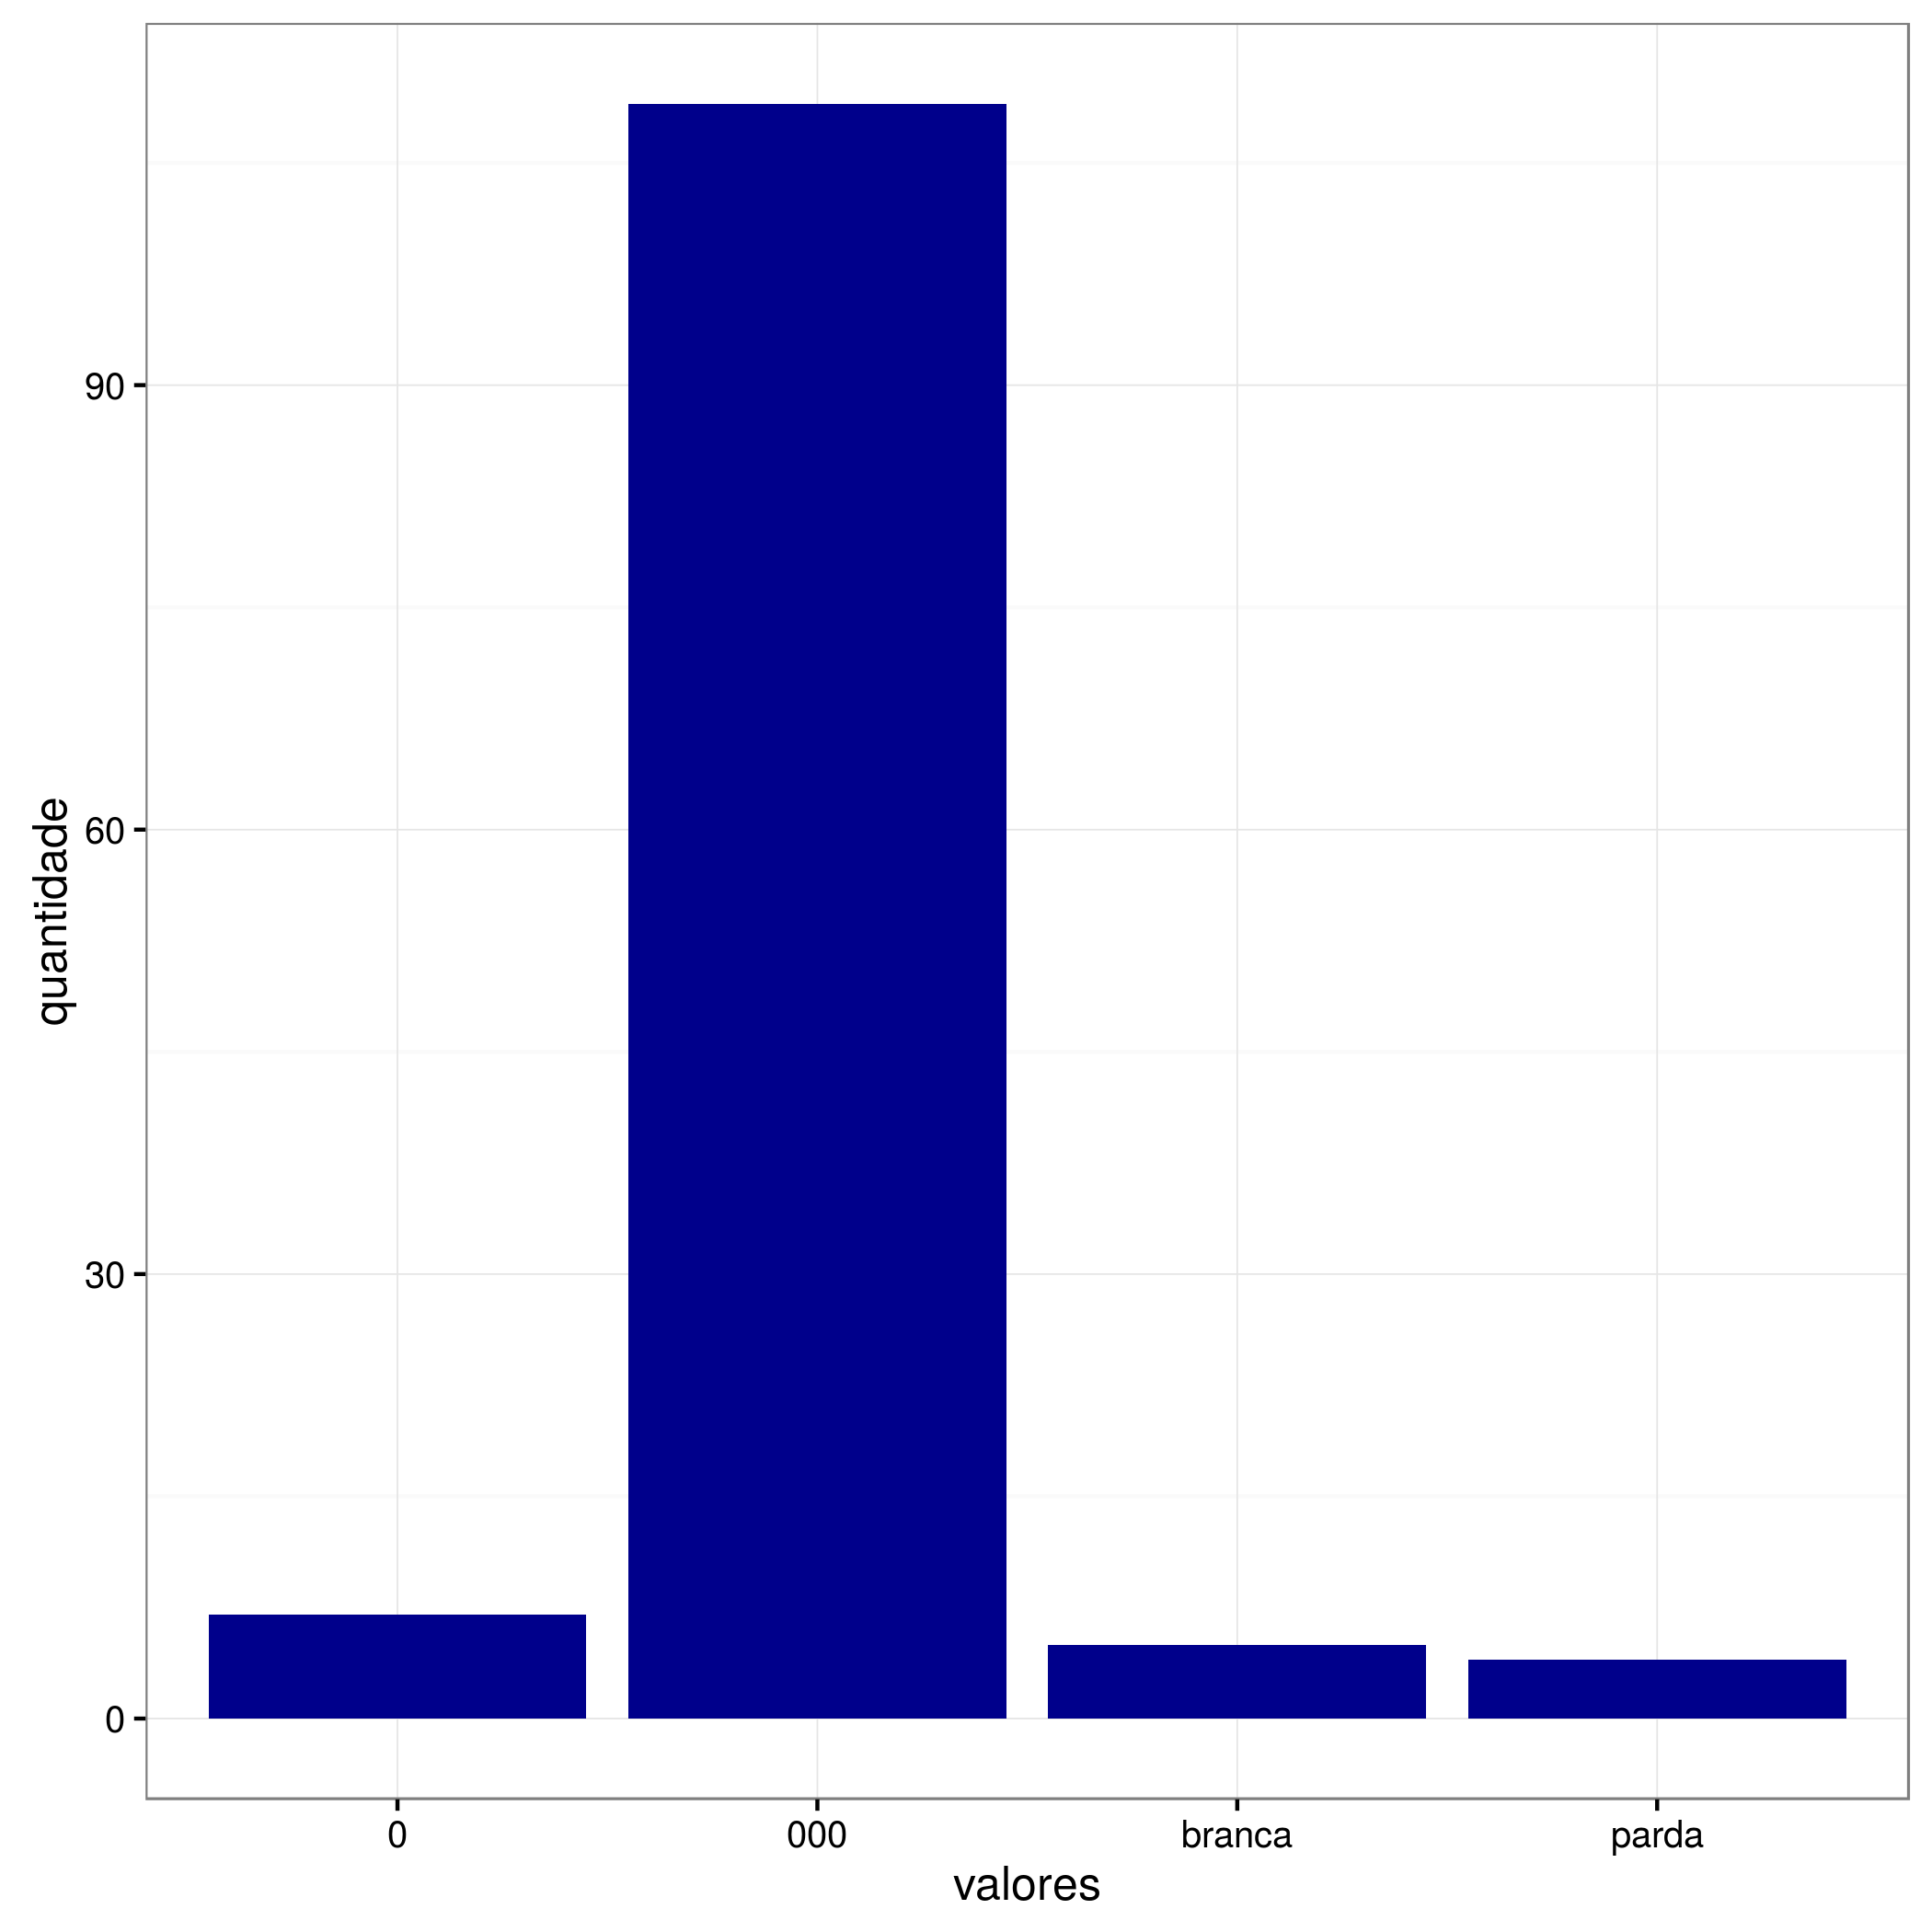
\includegraphics[width = 8cm]{race.png}
    \end{figure}
\end{frame}

\begin{frame}{Propriedades Gerais dos Dados - Curso}
    \begin{figure}[!ht]
        \centering
        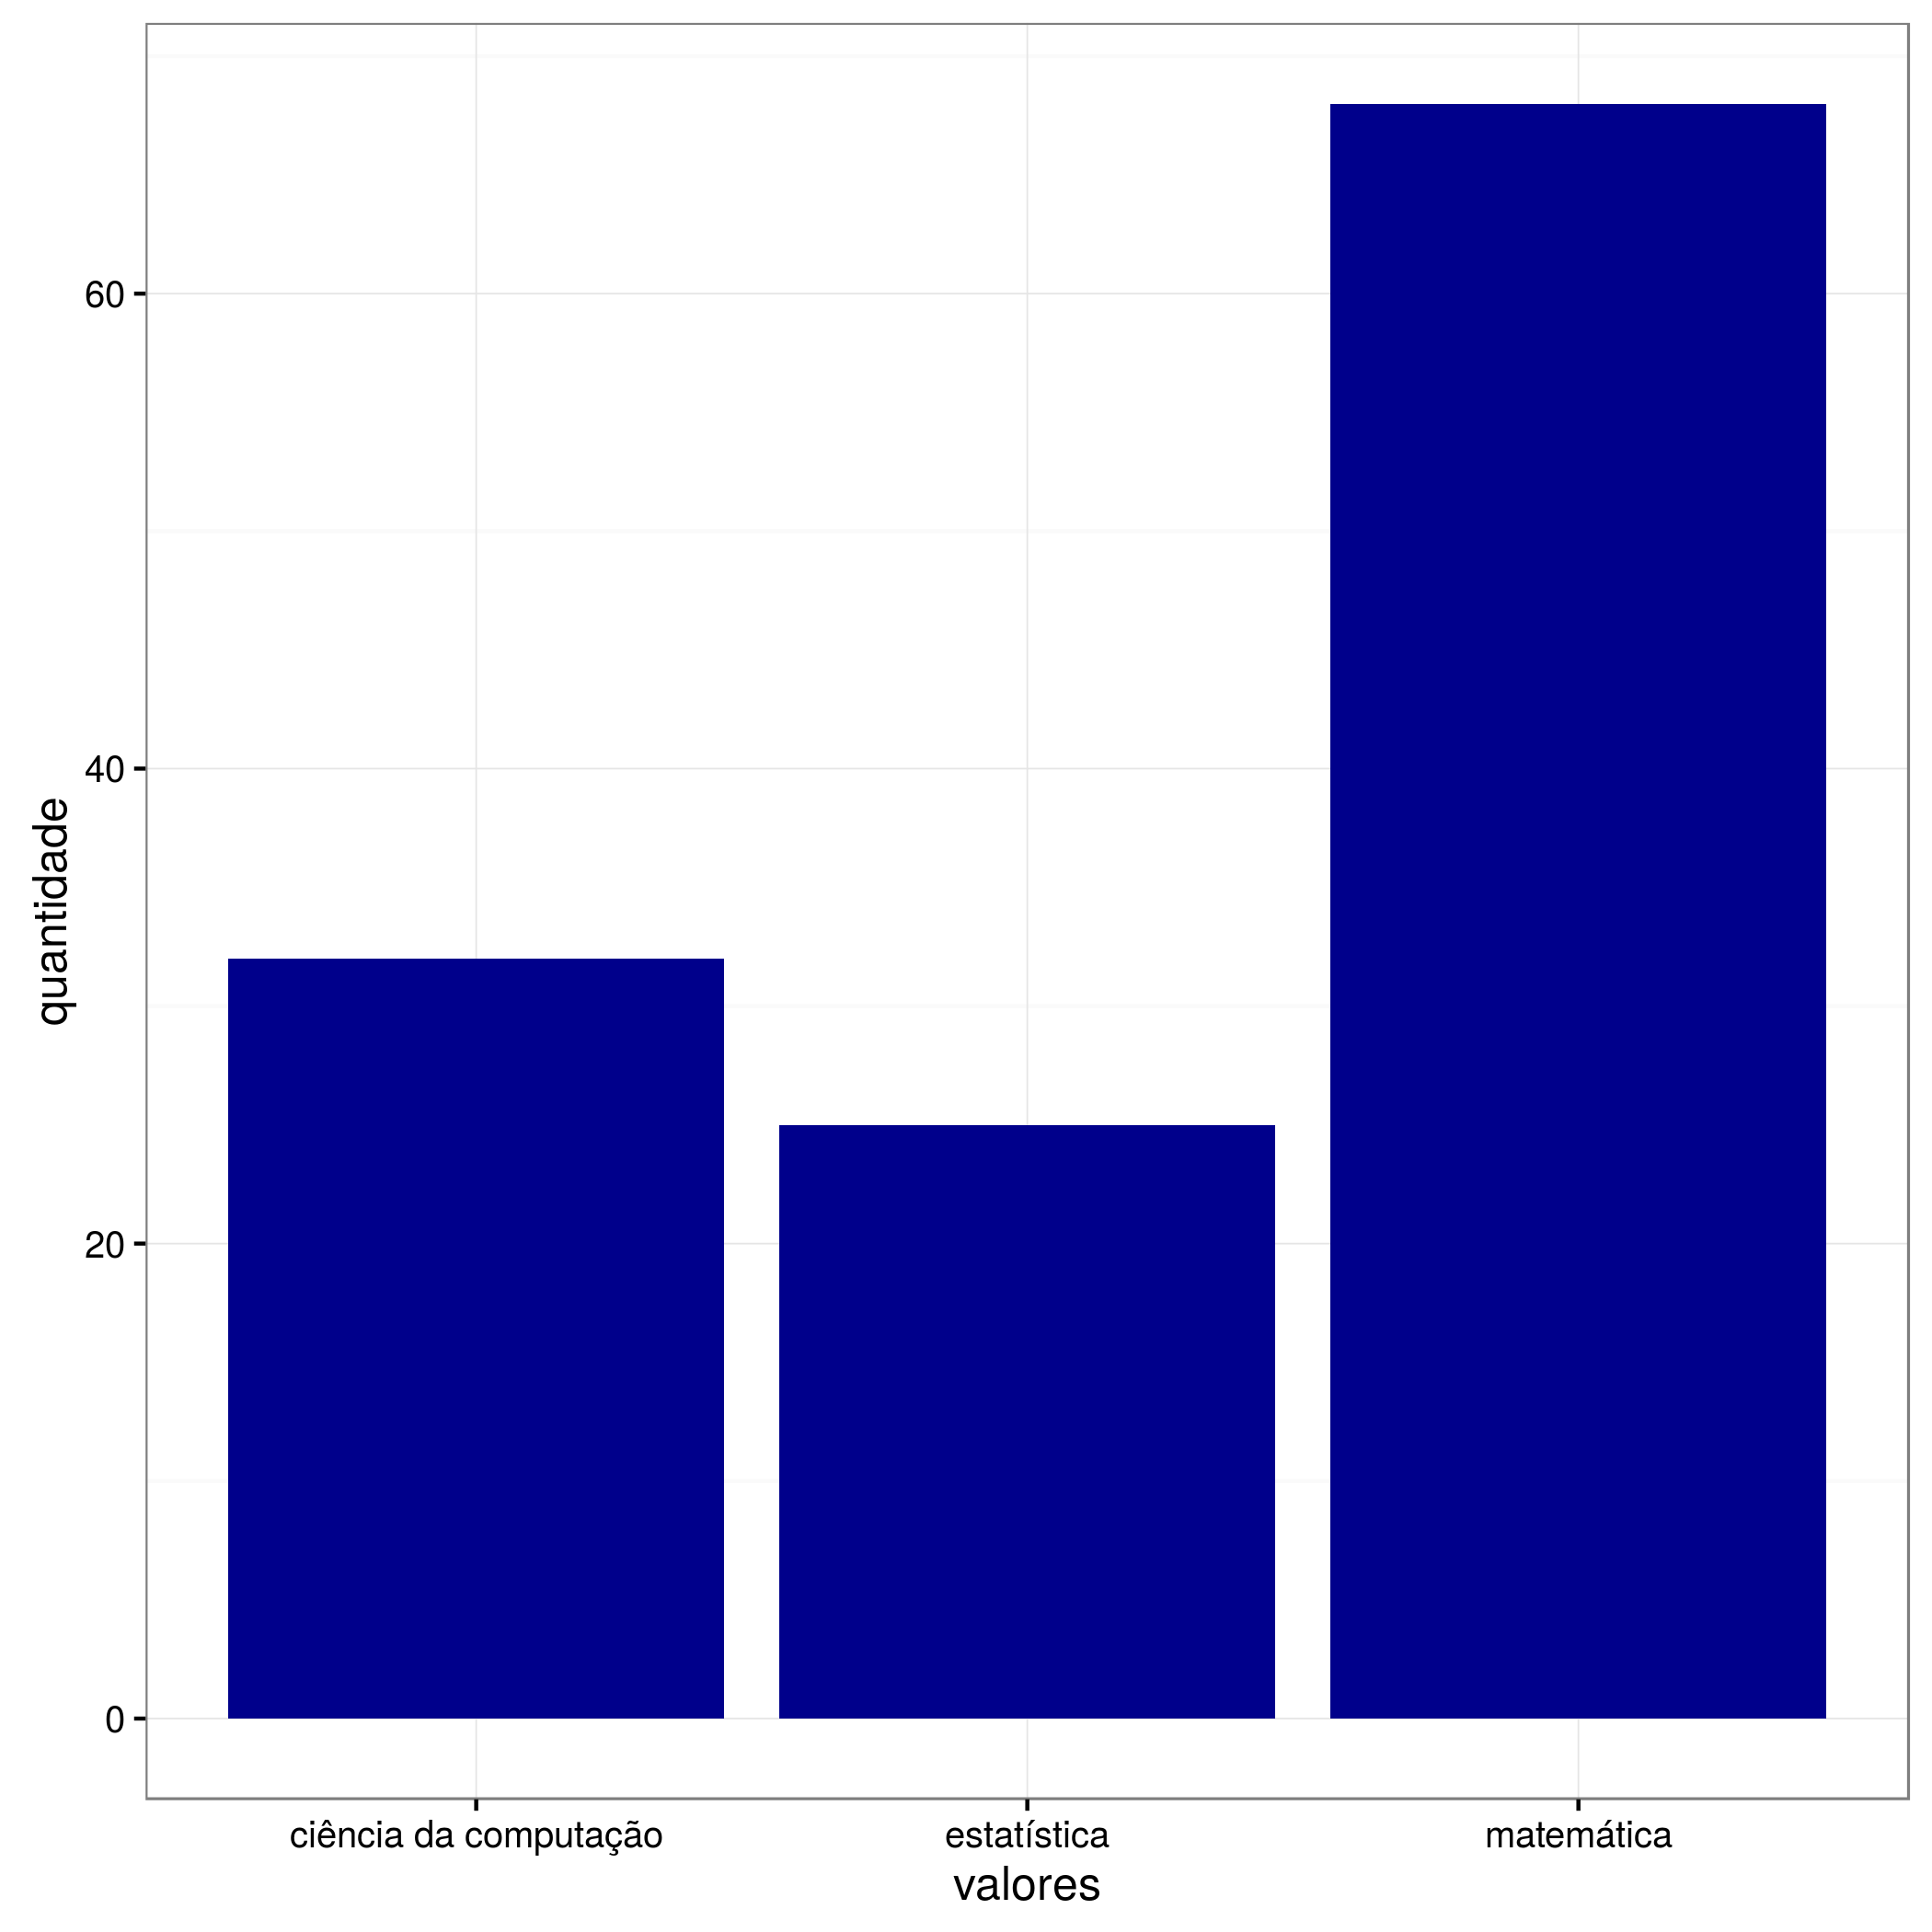
\includegraphics[width = 8cm]{course.png}
    \end{figure}
\end{frame}

\begin{frame}{Propriedades Gerais dos Dados - Forma de Ingresso}
    \begin{itemize}[itemsep=3ex]
        \item <gráfico mostrando forma de ingresso>
    \end{itemize}
\end{frame}

\begin{frame}{Média de Menções Obtidas nas Disciplinas}
    \begin{figure}[!ht]
        \centering
        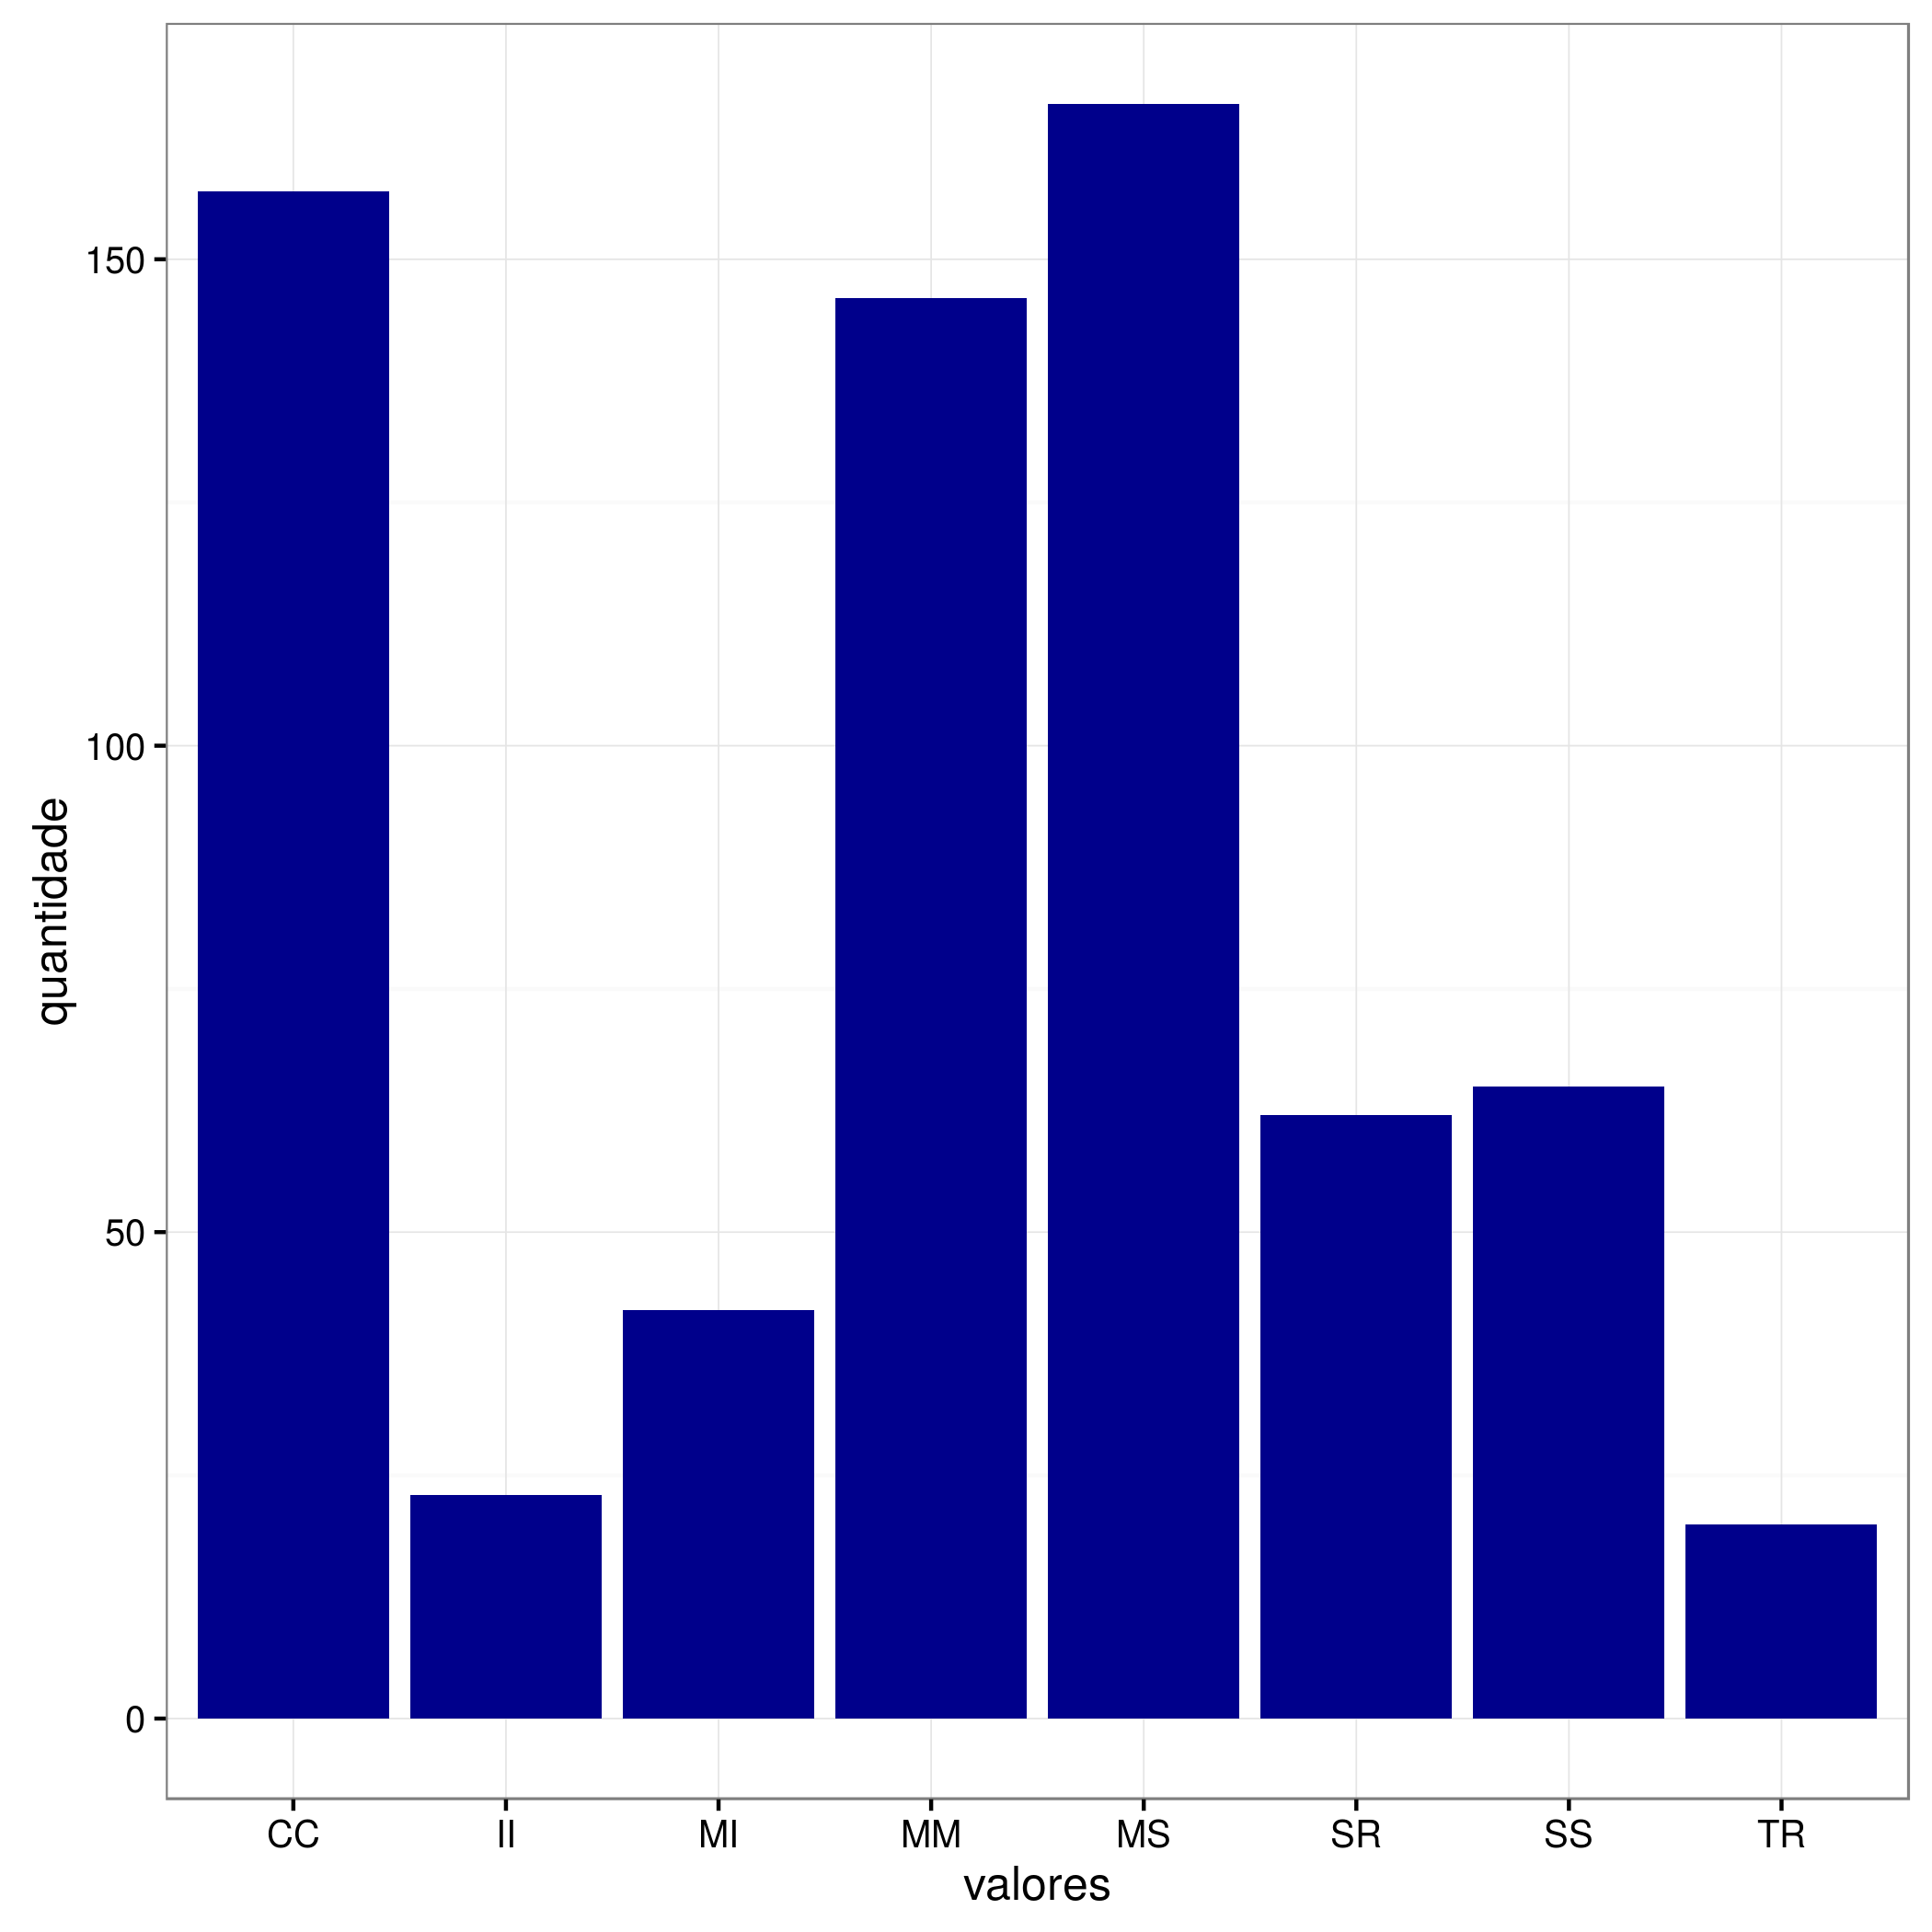
\includegraphics[width = 8cm]{grade.png}
    \end{figure}
\end{frame}



%\include{dados_derivados}

% bibliography
\begin{frame}{Referências}
\bibliographystyle{acm}
\bibliography{data_understanding}
\end{frame}

\end{document}

